\documentclass[journal]{vgtc}                % final (journal style)
%\documentclass[review,journal]{vgtc}         % review (journal style)
%\documentclass[widereview]{vgtc}             % wide-spaced review
%\documentclass[preprint,journal]{vgtc}       % preprint (journal style)
%\documentclass[electronic,journal]{vgtc}     % electronic version, journal

%% Uncomment one of the lines above depending on where your paper is
%% in the conference process. ``review'' and ``widereview'' are for review
%% submission, ``preprint'' is for pre-publication, and the final version
%% doesn't use a specific qualifier. Further, ``electronic'' includes
%% hyperreferences for more convenient online viewing.

%% Please use one of the ``review'' options in combination with the
%% assigned online id (see below) ONLY if your paper uses a double blind
%% review process. Some conferences, like IEEE Vis and InfoVis, have NOT
%% in the past.

%% Please note that the use of figures is not permitted on the first page
%% of the journal version.  Figures should begin on the second page and be
%% in CMYK or Grey scale format, otherwise, colour shifting may occur
%% during the printing process.  Papers submitted with figures on the
%% first page will be refused.

%% These three lines bring in essential packages: ``mathptmx'' for Type 1
%% typefaces, ``graphicx'' for inclusion of EPS figures. and ``times''
%% for proper handling of the times font family.

\usepackage{mathptmx}
\usepackage{graphicx}
\usepackage{times}
\usepackage{amsmath}

%% We encourage the use of mathptmx for consistent usage of times font
%% throughout the proceedings. However, if you encounter conflicts
%% with other math-related packages, you may want to disable it.

%% If you are submitting a paper to a conference for review with a double
%% blind reviewing process, please replace the value ``0'' below with your
%% OnlineID. Otherwise, you may safely leave it at ``0''.
\onlineid{0}

%% declare the category of your paper, only shown in review mode
\vgtccategory{Research}

%% allow for this line if you want the electronic option to work properly
\vgtcinsertpkg

%% In preprint mode you may define your own headline.
%\preprinttext{To appear in an IEEE VGTC sponsored conference.}

%% Paper title.

\title{Context Inconsistency Management \\in Pervasive Systems}

%% This is how authors are specified in the journal style

%% indicate IEEE Member or Student Member in form indicated below
\author{Samuel Esposito ~~~~~~~~~~~~ Alexander Jurjens}


%% Abstract section.
\abstract{Thanks to the pervasive computing paradigm more and more computer systems in utility buildings and industry are context-aware. They use a representation of the world they operate in to reduce the human-computer interaction necessary for their operation. Unfortunately reasoning based on contexts is not without flaws and context inconsistencies are the main reason for context-aware applications' incongruous behavior. Context consistency management is not adequately studied in existing literature and approaches for detecting and resolving context conflicts are not suited for pervasive computing~\cite{xu:2010:PCC}.

In this paper we present two complementary approaches for improving the mitigation of context inconsistencies. 
First we present partial constraint checking for timely identifying context inconsistencies at runtime. An extra constraint layer is added to the traditional ontology based context model and conflicts can be detected by locally checking partial constraints in the ontology. This dramatically improves performance compared to iterative evaluation of an entire ontology~\cite{xu:2010:PCC}.
Secondly we discuss the extension of the traditional ontology model with context life cycles to more accurately represent the environment of context-aware applications. This information can then be used to estimate the relative reliability of contexts in a conflict set and discard the contexts with lowest reliability~\cite{bu:2006:CCM}. 
Apart from resolving context conflicts it is also possible to represent inconsistencies into the context model itself~\cite{ko:2009:IOFO}. In this paper we present a use case in which we explore the possibilities of incorporating inconsistencies into context models using fuzzy ontologies.
} % end of abstract

%% Keywords that describe your work. Will show as 'Index Terms' in journal
%% please capitalize first letter and insert punctuation after last keyword
\keywords{Pervasive Computing, Ontology Model, Context Lifecycle, Inconsistency Resolution.}

%% Copyright space is enabled by default as required by guidelines.
%% It is disabled by the 'review' option or via the following command:
% \nocopyrightspace

%%%%%%%%%%%%%%%%%%%%%%%%%%%%%%%%%%%%%%%%%%%%%%%%%%%%%%%%%%%%%%%%
%%%%%%%%%%%%%%%%%%%%%% START OF THE PAPER %%%%%%%%%%%%%%%%%%%%%%
%%%%%%%%%%%%%%%%%%%%%%%%%%%%%%%%%%%%%%%%%%%%%%%%%%%%%%%%%%%%%%%%%

\begin{document}

%% The ``\maketitle'' command must be the first command after the
%% ``\begin{document}'' command. It prepares and prints the title block.

%% the only exception to this rule is the \firstsection command
\firstsection{Introduction}

\maketitle

In pervasive computing, contexts are used to make applications perform a certain action. Contexts can be seen as pieces of environmental information, which the applications depend on. Sometimes contexts are not consistent due to cross reads and misreads. The correctness of the contexts can be checked by evaluating the consistency constraints associated to them. There are multiple ways to check for consistency constraints. Constraint checking techniques are split up in two classes: Non-incremental checking and incremental checking. Incremental checking also consists of two classes: Entire Constraint Checking and Partial Constraint Checking. Once inconsistent contexts have been detected, an algorithm can be used to select the correct contexts. The algorithms use specific data structures, like ontology models, in order to resolve the inconsistencies. However, certain conflict resolving algorithms are too slow for use in practice. This paper describes a way to use an ontology model in combination with the Partial Constraint Checking algorithm in order to detect context inconsistencies fast enough, such that it can be used in practice. Another approach to handling context inconsistencies is representing them into the context model, as opposed to resolving them. This can be done efficiently by using fuzzy ontologies in a tree like structure, as we show in a use case.

\section{Related Work}
Pervasive or ubiquitous computing is a fast-developing discipline that has been receiving increasing attention from both researchers and software developers~\cite{xu:2010:PCC}. In the past decade, many context-aware systems have been developed, ranging from smart room environments to warehouse and supply chain management systems. A lot of effort has been put into building middleware infrastructures that handle vast amounts of sensory data and extract the context information relevant for pervasive applications. Examples of such systems are CoBrA~\cite{1276865} and CORTEX~\cite{1276875}. Various modeling approaches have been proposed for capturing context information, of which the ontology based context model appears to be most promising for most pervasive applications~\cite{bu:2006:CCM}.

Context management for consistency however has not been adequately studied in the existing literature. None of the studies on context-awareness discusses a way for detecting context inconsistencies for reliable pervasive computing~\cite{xu:2010:PCC, bu:2006:CCM}. Even though other disciplines as artificial intelligence and software engineering conducted relate research, it does not provide adequate support for context inconsistency detection in ubiquitous computing. In addition the strategies proposed in literature for resolving context conflicts are not suited for pervasive computing. Some are based on assumptions that may not apply to general pervasive environments. Other require human participation for conflict resolution, which is usually expensive and slow for pervasive computing~\cite{xu:2010:PCC}. Finally no research has been done on the potential of fuzzy ontologies to represent context inconsistencies in the environment instead of trying to resolve them~\cite{ko:2009:IOFO}.

In this article we aim at putting a milestone for context management by presenting an efficient inconsistency detection algorithm based on a constraint language extending the traditional ontology based context model~\cite{xu:2010:PCC}. In addition we put forward a conflict resolution algorithm which is based on a context reliability heuristic~\cite{bu:2006:CCM}. Finally the use of fuzzy ontologies representing context inconsistencies as a promising alternative to conflict resolution is explored.

\section{Partial Constraint Checking}
Constraint checking techniques have been extensively studied in software engineering. Existing constraint checking algorithms focus on checking software artifacts that do not change rapidly or frequently~\cite{xu:2010:PCC}. Context-aware applications require more efficient algorithms because they use a huge set of contexts, which can change very rapidly and frequently (in the range of milliseconds). An inefficient software solution for this does not only require massive computing power, but interestingly also induces a higher inconsistency detection miss rate. Because of the computing delay conflicting contexts slip through the context buffer before they are detected by the software~\cite{xu:2010:PCC}. One example of an inefficient approach is non-incremental checking: whenever there is a change in the set of software artifacts these artifacts are each checked against the entire set of consistency constraints to find out all detectable inconsistencies. An improvement to this would be incremental checking: only a subset of all constraints are checked, namely those that are affected by the specific change in the artifact set. But the real merit of Xu et \textit{al.} was replacing the traditional entire constraint checking approach by partial constraint checking based on a consistency computation tree~\cite{xu:2010:PCC}. Their idea is that constraints can be represented as trees with nodes for logical operations and leaves for specific properties of contexts or context sets. Whenever a context is added to or deleted from a context set in time, the branch corresponding to this context can respectively be added to or deleted from the tree (see Fig.~\ref{fig:cct}). 
\begin{figure}[htb]
  \centering
  \includegraphics[width=3.5in]{cons_comp_tree}
  \caption{Consistency Computation Tree: branches can be added or deleted to represent changes in a context set. Source:~\cite{xu:2010:PCC}}
  \label{fig:cct}
\end{figure}
Because intermediate values are retained in the tree nodes after calculation they can be reused whenever the tree changes. More specifically, when a branch is added, only the values of the new branch itself and of the nodes from the branch top to the tree root need to be calculated. When a branch is deleted, only the values for the nodes from the branch top to the tree root have to be recalculated. 

With their partial constraint checking algorithm Xu et \textit{al.} attained a time complexity between $O(n)$ in the worst case and $O(1)$ in the best case when a context is added to the set and $O(1)$ when a context is removed. Compared to traditional constraint checking with an overall complexity of $O(n)$, this is a dramatical improvement. In their experiments Xu et \textit{al.} showed their performance is 15 times better than the traditional approach and in a case study the inconsistency miss rate dropped from $52.2\%$ in traditional checking to $0.1\%$ with partial checking~\cite{xu:2010:PCC}.

\section{From Ontology to CCT}
As stated above the Partial Constraint Checking (PCC) algorithm is much faster than Entire Constraint Checking due to the fact that a Consistency Computation Tree (CCT) is used to store the constraints belonging to a (set of) context(s). We also stated that the ontology based context model is the most promising type of model to capture context information. Although the context model appears as a tree (see Fig. \ref{fig:ont}), the PCC algorithm cannot be directly applied to it.

\begin{figure}[htb]
  \centering
  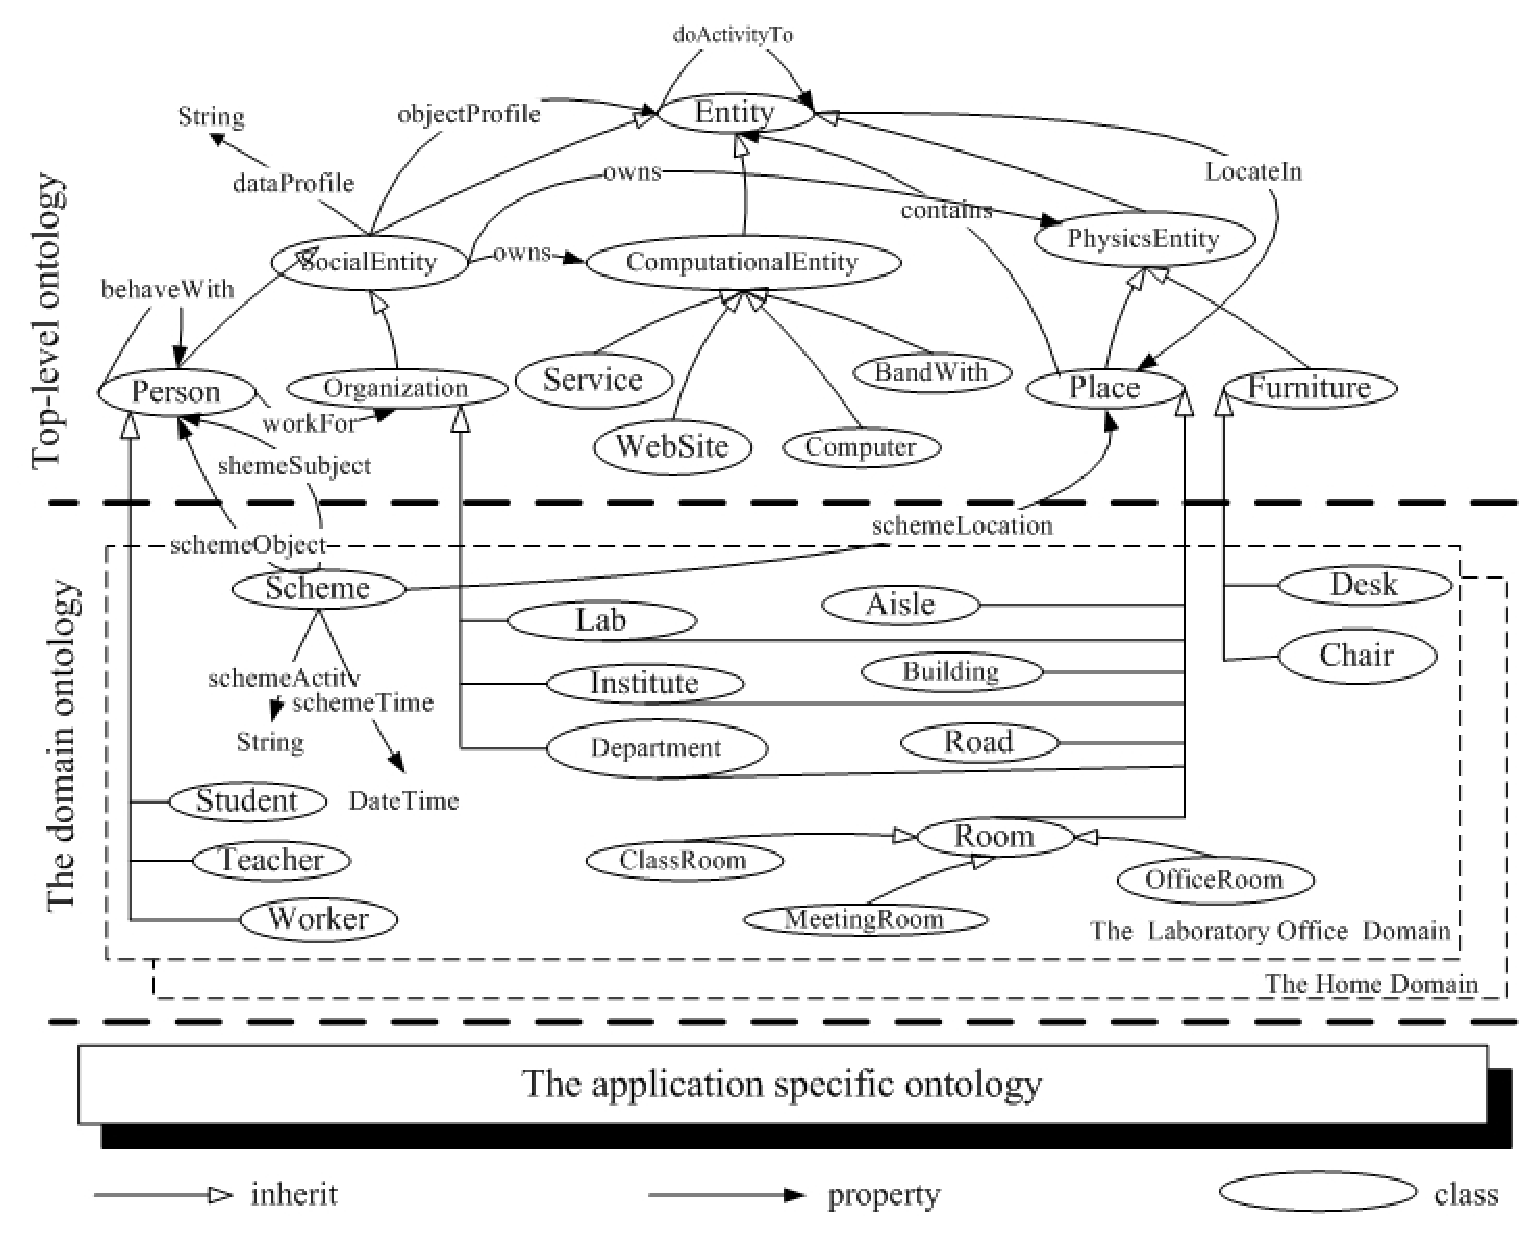
\includegraphics[width=3.5in]{Ontology.eps}
  \caption{An example of an ontology based context model Source:~\cite{bu:2006:CCM}}
  \label{fig:ont}
\end{figure}

The model is actually a part of a larger ontology, but it is sufficient for this section. Now it needs to be transformed into a CCT for PCC. With a CCT the main focus should be on the context set of a single entity in the model. The transformation itself can be done automatically with a depth-first search algorithm, but there is no such algorithm available at this time. However, we can give a few examples of the CCT based on this ontology model. The context set of the entity \textit{Student} will be focused on. Lets say that the entity \textit{Student} is located in the \textit{Place} entity \textit{Road}, then the CCT will look as the upper tree in Fig. \ref{fig:cct1}.

\begin{figure}[htb]
  \centering
  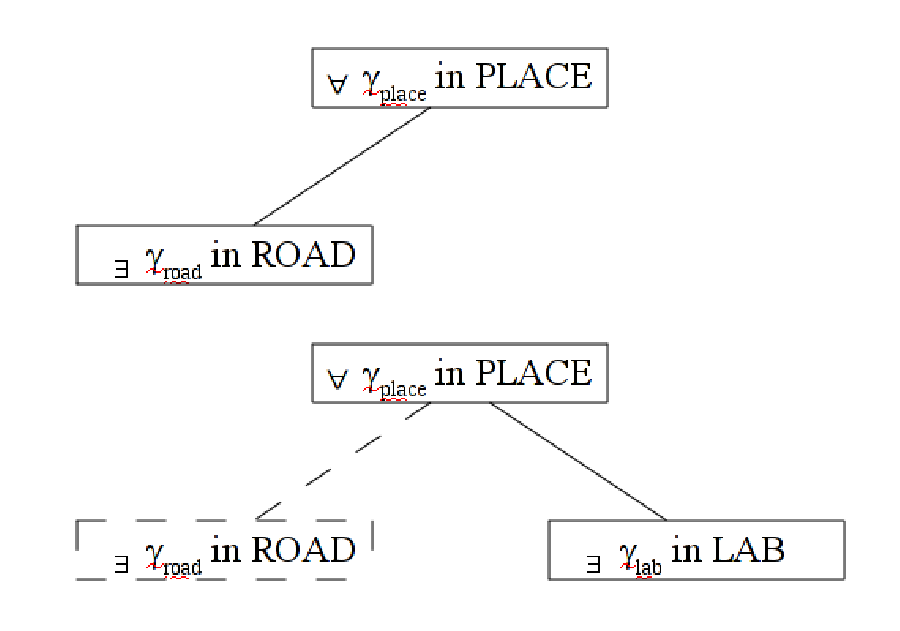
\includegraphics[width=3.5in]{smallCCT1.eps}
  \caption{The CCTs of \textit{Student}}
  \label{fig:cct1}
\end{figure}

If the system suddenly decides that \textit{Student} is located in a \textit{Lab}, then the tree will be updated to the lower tree. Note that the system can decide in a multitude of ways that \textit{Student} is located in the \textit{Lab} by for example invalidating the earlier constraint branch after a certain amount of time or by for example basing the new \textit{Place} on the information in a new context set. Also note that the leaf of a branch cannot contain an entity that is not available in the context model. So \textit{Student} cannot be located in, for example, \textit{Car}, because it is not part of the model. Even if the location in a context would be \textit{Car}, then the system would consider the location as an inconsistency in the context and detect it very quickly with PCC.

\section{Context Inconsistency Resolution}
Now that we have an efficient method for detecting inconsistencies the task of resolving the conflicts remains. As discussed above the strategies for conflict resolution in literature are not well suited for pervasive computing because their assumptions do not apply or they require human participation~\cite{xu:2010:PCC}. What is really needed is an algorithm that in the case of a conflict between two or more contexts decides which context has the highest reliability and retains that context. Bu et \textit{al.} show us that this is possible through extending the ontology based context model with additional information about the context's status and temporal properties~\cite{bu:2006:CCM}. More specifically they propose an algorithm that for every conflict set retains the context with the highest \textit{relative frequency}: frequency of context updates relative to update interval and context age (see Fig.~\ref{fig:cir}). 
\begin{figure}[htb]
  \centering
  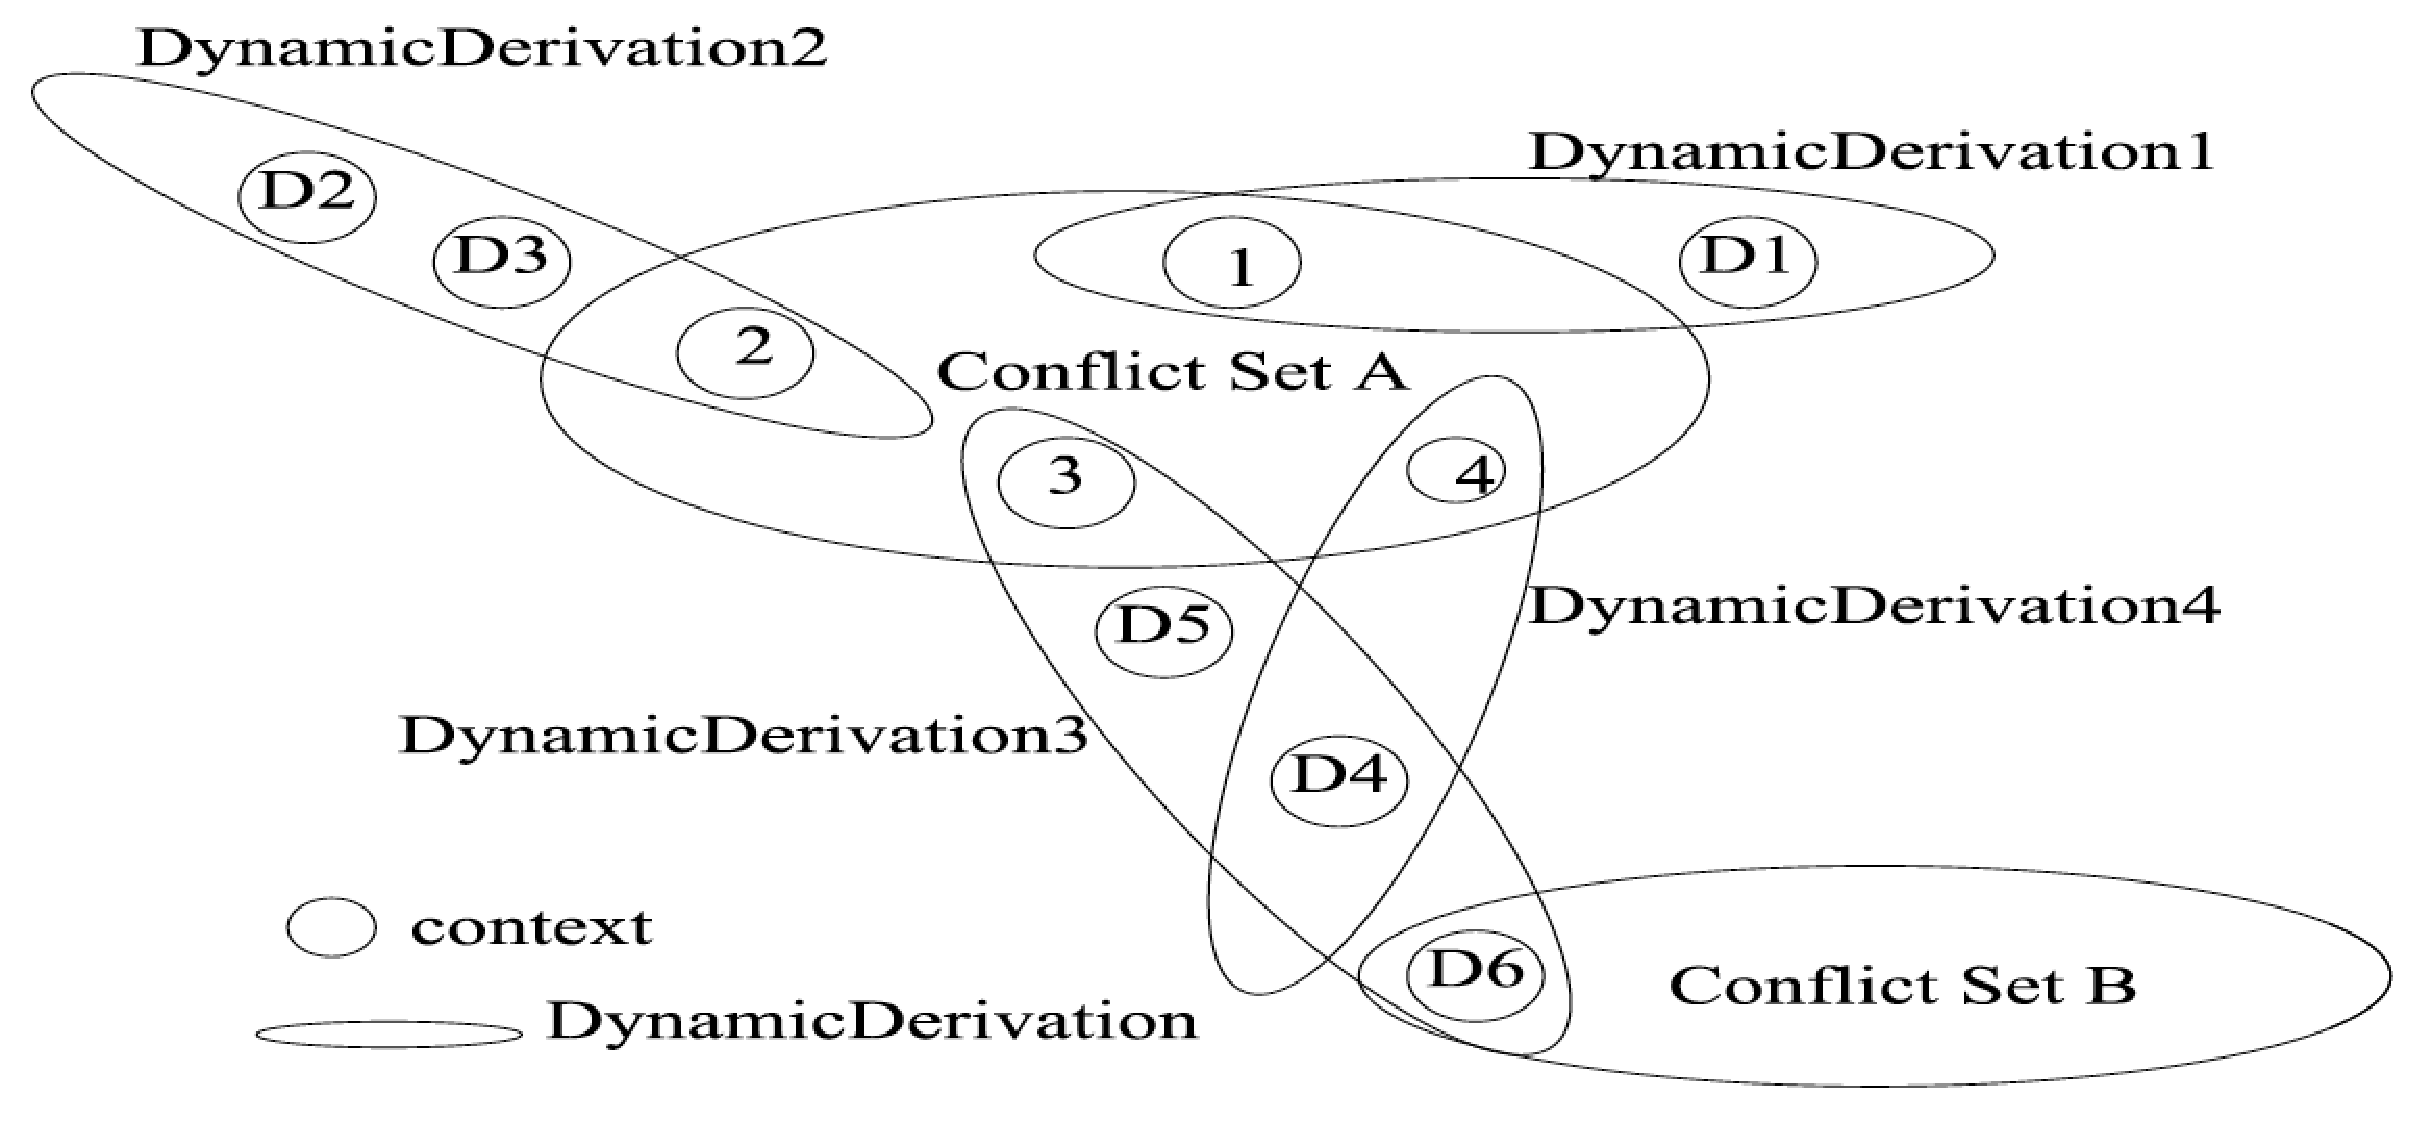
\includegraphics[width=3.5in]{cir}
  \caption{Context inconsistency resolution in action. Source:~\cite{bu:2006:CCM}}
  \label{fig:cir}
\end{figure}
This is based on the assumption that contexts that are most stably perceived by a system are most likely to be correct. This assumption is applicable to most of the environments in which pervasive systems run and is applied in many domains as a domain specific approach~\cite{xu:2010:PCC}.

\section{Fuzzy Ontologies}
In pervasive computing traditionally first order logic is used to model the environment of an application. This results in a so called ontology based context model. Every observation that does not exactly fit in this model results into a conflict. This conflict can lead to misadjusted behavior in applications unless they are timely detected and resolved~\cite{xu:2010:PCC}. Because it is impossible to perfectly model the un-predictive environment in which context-aware applications run, it would be nice if the context model was more resilient to unexpected observations. As we illustrate in the case study below, this can be obtained by using fuzzy ontologies.
\subsection{Case Study}
Suppose we want to build a context-aware application that has certain notion of teacher's activities to assist them in the best possible way (for instance automatically opening slides when a lecture starts). In the traditional approach we could build an ontology specifying where lectures take place and that a lecture starts when the teacher appears at the lectern. If now an unpredicted observation is made (sensor cross read or teacher momentarily leaves the room), an inconsistency occurs that has to be resolved for the application to proceed with normal operation. In the fuzzy ontology approach these unpredictable events can simply be modeled so that the ontology is more robust and always yields the most apt interpretation of the environment without conflict resolution. A simplified example of such an ontology is depicted in Fig.~\ref{fig:fuzzy}.
\begin{figure}[htb]
  \centering
  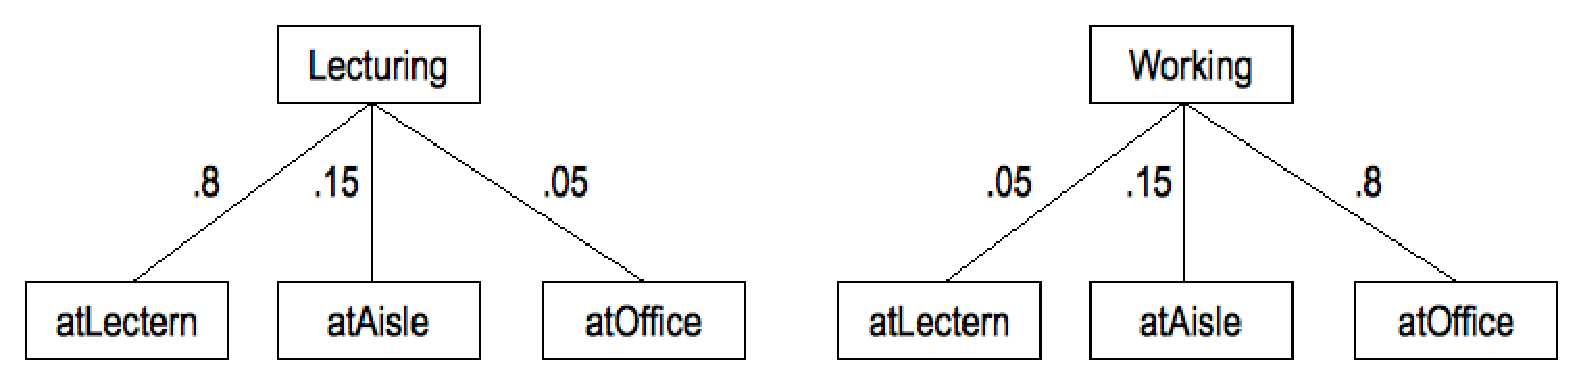
\includegraphics[width=3.5in]{fuzzy}
  \caption{Fuzzy ontology specifying teachers activities and their most probable location.}
  \label{fig:fuzzy}
\end{figure}
Using this fuzzy ontology the relative probability of each specified higher-level context can be calculated from the contexts in the observation window. For instance the observation sequence [$L_1$, $L_2$, $L_3$, $A_1$, $A_2$] gives a relative probability of 0.9998 for `Lecturing' and 0.0002 for `Working', event though the observations are clearly conflicting, since the teacher clearly cannot be at the lectern and in the aisle at the same time. The sequence of [$L_1$, $A_1$, $A_2$, $O_1$, $O_2$] gives a 0.941 probability for `Working' and 0.059 for `Lecturing', even though the teacher strictly spoken cannot be at the lectern and in the office at the same time (see appendix for exact calculations). 

\subsection{Results}
Regardless of any inconsistencies in the observed contexts a fuzzy ontology always yields the most probable higher-level context without the need for conflict detection and resolution.

Interestingly a fuzzy ontology has some tree-like structure that allows for very efficient incremental partial probability calculation (PPC). The probability of a higher-level context is calculated by simply multiplying the probabilities of the observed contexts. When a new context is added to the observation window, the intermediate calculation result stored at a node (the root in our case study) can simply be multiplied by the probability of the new observation in order to obtain the updated probability for a higher-level context. When a context disappears from the observation window, the intermediate result can simply be divided by the context's probability to obtain an updated probability for a higher-level context. 

Note that it is possible to extend the simple fuzzy ontology from the use case by specifying start and transition probabilities for the higher-level contexts, just as hidden Markov models\footnote{http://en.wikipedia.org/wikiHidden\_Markov\_model} do, and other information such as the expected lecture time window (fuzzified of course~\cite{Buckley1995245}).

\section{Discussion}
In this article we started with presenting partial constraint checking: an efficient algorithm for timely detecting inconsistencies in huge sets of contexts which change frequently. Partial constraint checking was 15 times as efficient as the traditional greedy approach and reduced the conflict detection miss rate from 52.2\% to 0.1\%. This algorithm is clearly a dramatic improvement of the traditional approach and vital to any context aware application that has to handle frequently generated contexts.

Then we have shown examples of CCTs of entities in an ontology based context model. We have not shown an algorithm on how to do this efficiently as we don't know the formal definition of OWL at this point in time. However, with the definitions of OWL one can create a depth-first search algorithm that transforms an ontology in multiple CCTs (one for each leaf entity in the model).

After that we shed light on ways to resolve the detected conflicts and discussed a context inconsistency resolution algorithm that estimates the reliability of conflicting contexts and only retains the most reliable context from every conflict set. Using this algorithm allows for timely conflict resolution at runtime without the need for human participation. The algorithm is a valuable addition to the research on conflict resolution in pervasive computing, but when applying it one has to verify the aptness of the heuristic used for context reliability estimations in the domain at hand. In particular the assumption that contexts with the highest relative frequency are most reliable has to apply in the domain.

Finally the use of fuzzy ontologies for modeling the environment of context-aware applications seems promising. By incorporating possible inconsistencies in the model the need for context inconsistency management vanishes, vastly reducing the complexity of the used middleware. Fuzzy ontologies always yield the most probable higher-level contexts, regardless of the inconsistencies in the observed context set. In addition the calculation of the probabilities in a fuzzy ontology has great potential for optimization by using incremental partial probability calculation. 
When using fuzzy ontologies one however has to take into account the required training of the system for obtaining well defined probabilities in the context model. 

\section{Conclusion}
In conclusion we can say that the partial constraint checking algorithm can dramatically improve the performance of context-aware applications where context consistency management is needed. With this performance improvement we get an impressive reduction of missed context inconsistencies for free. The context inconsistency resolution algorithm is a good solution in most domains for timely resolving context conflicts without human intervention. The fuzzy ontology approach seems a promising alternative to traditional context modeling but needs extensive further research in order to determine its real value in context-aware applications.

\bibliographystyle{abbrv}
%%use following if all content of bibtex file should be shown
%\nocite{*}
\bibliography{paper}
\newpage
\appendix
\section{Fuzzy Ontology Calculations}
Observed Context Set 1: $[L_1, L_2, L_3, A_1, A_2]$
\begin{align}
                          Lecturing &= .8 * .8 * .8 * .15 * .15 * c_1\\
                                    &= .01152 * c_1\\
                                    &= 0.9998\\
                            Working &= .05 * .05 * .05 * .15 * .15 * c_1\\
                                    &= 0.000002813 * c_1\\
                                    &= 0.0002
\end{align}
Observed Context Set 2: $[L_1, A_1, A_2, O_1, O_2]$
\begin{align}
                          Lecturing &= .8 * .15 * .15 * .05 * .05 * c_2\\
                                    &= 0.000045 * c_2\\
                                    &= 0.059\\
                            Working &= .05 * .15 * .15 * .8 * .8 * c_2\\
                                    &= 0.00072 * c_2\\
                                    &= 0.941
\end{align}
\end{document}
